\documentclass[notes=hide,hyperref={dvipdfmx,pdfpagelabels=false}]{beamer}
\title{Einführung in Sage - Einheit 9}
\subtitle{Strings, interaktive Grafiken, GeoGebra, Komplexe Beispiele}
\mode<article>
{
  \usepackage{fullpage}
  \usepackage{pgf}
  \usepackage[xetex]{hyperref}
  \setjobnamebeamerversion{beamer}
}

\mode<presentation>
{
  %\usetheme{Frankfurt}
 %\usetheme{My}
  \usetheme{Madrid}
  % or ...
%\usecolortheme{seagull}
  %\setbeamercovered{transparent}
  %\setbeamercovered{dynamic}
  % or whatever (possibly just delete it)
}
\usenavigationsymbolstemplate{}
\usefonttheme{structurebold}
\usepackage{multimedia}
%\usepackage{tikz}
\usepackage{fontspec,xunicode,xltxtra}

%\usepackage{polyglossia}
%\setdefaultlanguage[spelling=new, latesthyphen=true]{german}
%\setsansfont{DejaVu Sans}
%\setsansfont{Verdana}
%\setsansfont{Arial}
%\setromanfont{Linux Libertine O}
%\setsansfont{Linux Biolinum O}

\setbeamertemplate{footline}
{
\leavevmode
%\hbox{\begin{beamercolorbox}[wd=.5\paperwidth,ht=2.5ex,dp=1.125ex,
%leftskip=.3cm plus1fill,rightskip=.3cm]{author in head/foot}%
%    \usebeamerfont{author in head/foot}\insertshortauthor
%  \end{beamercolorbox}%
%  \begin{beamercolorbox}[wd=.5\paperwidth,ht=2.5ex,dp=1.125ex,leftskip=.3cm,
%rightskip=.3cm plus1fil]{title in head/foot}%
%    \usebeamerfont{title in head/foot}\insertshorttitle\hfill

\hfill\insertframenumber  \hspace{3pt}

%\inserttotalframenumber
%\hspace*{2ex}
%  \end{beamercolorbox}}%
  \vskip3pt%
}

\usepackage[ngerman]{babel}
\selectlanguage{ngerman}

%
% math/symbols
%
\usepackage{amssymb}
\usepackage{amsthm}
% \usepackage{latexsym}
\usepackage{amsmath}
%\usepackage{amsxtra} %Weitere Extrasymbole
%\usepackage{empheq} %Gleichungen hervorheben
%\usepackage{bm}
 %\bm{A} Boldface im Mathemodus

\usepackage{cellspace}
\setlength{\cellspacetoplimit}{2pt}
\setlength{\cellspacebottomlimit}{2pt}

%%%%%%%%%%%%%%%%%% Fuer Frames [fragile]-Option verwenden!
%Programm-Listing
%%%%%%%%%%%%%%%%%%
%Listingsumgebung fuer verbatim
%Grauhinterlegeter Text
%Automatischer Zeilenumbruch ist aktiviert
\usepackage{listings}
\definecolor{lgray}{gray}{0.80}
%\lstset{backgroundcolor=\color{lgray}, frame=single, basicstyle=\ttfamily, breaklines=true}
\lstnewenvironment{sage}{\lstset{backgroundcolor=\color{lgray},language=Python, emphstyle=\color{red}, frame=single, basicstyle=\ttfamily, breaklines=true,mathescape =true,escapechar=§}}{}


\usepackage{mydef}
%\usepackage{cmap} % you can search in the pdf for umlauts and ligatures
\usepackage{colonequals} %corrects the definition-symbols \colonequals (besides others)
\title{Einführung in Sage}
%
%\subtitle{Disputation} % (optional)

\author{Jochen Schulz}
% - Use the \inst{?} command only if the authors have different
%   affiliation.

\institute{Georg-August Universit\"at G\"ottingen \pgfimage[height=0.5cm]{../figures/unilogo3}}
% - Use the \inst command only if there are several affiliations.
% - Keep it simple, no one is interested in your street address.

\date{\today}

\subject{Sage}
% This is only inserted into the PDF information catalog. Can be left
% out. 

% If you have a file called "university-logo-filename.xxx", where xxx
% is a graphic format that can be processed by latex or pdflatex,
% resp., then you can add a logo as follows:

%\logo{\pgfimage[height=0.5cm]{figures/unilogo3}}


% Delete this, if you do not want the table of contents to pop up at
% the beginning of each subsection:

\AtBeginSection[]
{
  \begin{frame}<beamer>
    \frametitle{Aufbau}
    \tableofcontents[currentsection,currentsubsection]
  \end{frame}
}

\AtBeginSubsection[]
{
  \begin{frame}<beamer>
    \frametitle{Aufbau}
    \tableofcontents[currentsection,currentsubsection]
  \end{frame}
}



%%%%%%%%%%%%%%%%%%%
%Neue Definitionen
%%%%%%%%%%%%%%%%%%%

%Newcommands
\newcommand{\Fun}[1]{\mathcal{#1}}      %Mathcal fuer Funktoren
\newcommand{\field}[1]{\mathbb{#1}}     %Grundkoerper ?? in mathds

\newcommand{\A}{\field{A}}              %Affines A
\newcommand{\C}{\field{C}}              %Complexes C
\newcommand{\Fp}{\field{F}_{\!p}}       %Endlicher Koerper mit p Elementen
\newcommand{\Fq}{\field{F}_{\!q}}       %Endlicher Koerper mit q Elementen
\newcommand{\Ga}{\field{G}_{a}}         %Add Gruppenschema
\newcommand{\K}{\field{K}}              %Generischer Koerper 
\newcommand{\N}{\field{N}}              %Nat Zahlen
\newcommand{\Pj}{\field{P}}             %Projektives P
\newcommand{\R}{\field{R}} 		%Reelle Zahlen
\newcommand{\Q}{\field{Q}}              %Rationale Zahlen  
\newcommand{\Qt}{\field{H}}             %Quaternionen 
\newcommand{\V}{\field{V}}              %Vektorbuendel V
\newcommand{\Z}{\field{Z}}              %Ganze Zahlen

\newcommand{\fdg}{\;|\;}                 %fuer die gilt

%Operatoren
\DeclareMathOperator{\Abb}{Abb}
%\usepackage{sagetex}

\begin{document}
\lstset{basicstyle={\lstbasicfont\footnotesize}}


\begin{document}
\maketitle

\begin{frame}{Aufbau}
\tableofcontents
\end{frame}

\begin{frame}{Klausur}
 \begin{itemize}
\item Zeit: 9.03.2012 von 10:00 - 11:30
\item  Ort: HS1 (A bis J) und AudiMax (K bis Z)
\item  Hilfsmittel: Schreibgerät(e) und Unterlagen in Papierform
\item  Studenten-Ausweis mitbringen
\item Schreibweisen der Art $x^2$ oder $xy$ sind ok, solange klar ist was gemeint ist.
%\item  Ab 10:30 keine vorzeitige Abgabe möglich
\end{itemize}

\end{frame}

%===================================================
\section{Umgang mit Strings}
%==================================================


\begin{frame}[Sage]
    \begin{center}
        \url{https://sage.math.uni-goettingen.de/home/pub/54/}
    \end{center}
\end{frame}

\section{Interaktive (grafische) Elemente}

\begin{frame}[Sage]
    \begin{center}
        \url{https://sage.math.uni-goettingen.de/home/pub/55/}
    \end{center}
\end{frame}


\section{GeoGebra}

\begin{frame}[Sage]
    \begin{center}
        \url{https://sage.math.uni-goettingen.de/home/pub/56/}
    \end{center}
\end{frame}

%%%%%%%%%%%%%%%%%%%%%%%%%%%%%%%%%%%%%%%%%%
\section{Vertiefung Programmierung}
%%%%%%%%%%%%%%%%%%%%%%%%%%%%%%%%%%%%%%%%%%

\begin{frame}[fragile]{Größter gemeinsamer Teiler (ggT)}
Berechnung des ggT von natürlichen Zahlen $a$ und $b$ mit Hilfe des
euklidischen Algorithmus.
\bigskip

\textbf{Idee:} Es gilt:
\begin{enumerate}
 \item $ggT(a,b)=ggT(a,b-a)$ für $a<b$.
\item $ggT(a,b)=ggT(b,a)$.
\item $ggT(a,a)=a$.
\end{enumerate}

\textbf{Algorithmus:}

Wiederhole,  bis $a=b$
 \begin{itemize}
\item Ist $a>b$, so $a=a-b$.
\item Ist $a<b$, so $b=b-a$ 
\end{itemize}
\end{frame}

\begin{frame}[fragile]{ggT - Implementierung}
\begin{sagein}
def ggT(a,b):  
    """Bestimme den ggT von a und b"""
    while a<>b:
        if a>b:
            a = a-b
        else: 
            b = b-a
    return a
ggT(6,9)
\end{sagein}
\begin{sage}
3  
\end{sage}

\end{frame}




% %-----------------------------
% \subsection{Schleifen}
% %----------------------------
% 
% \begin{frame}[fragile]{Repeat}
% Neben \isage{for} ist durch  \isage{repeat} eine weitere Schleifenvariante gegeben:
% \begin{sage}
% x:=1.1:
% repeat
%   i:=x; x:=i^2; print(i,x)
% until x>100 end_repeat:
% \end{sage}
% Die Befehle zwischen \isage{repeat} und \isage{until} werden so lange
% wiederholt, bis die Bedingung (hier $x>100$) wahr wird.
% \end{frame}
% 
% \begin{frame}[fragile]{while}
% So ähnlich wie die \isage{repeat}-Schleife funktioniert die
% \isage{while}-Schleife. 
% \begin{sage}
% x:=2:
% while x<=100 do
%  i:=x; x:=i^2; print(i,x)
% end_while:
% \end{sage}
% Die Befehle zwischen \isage{while} und \isage{end_while} werden so lange
% wiederholt, wie die Bedingung (hier $x<=100$) wahr ist.
% \end{frame}
% 
% \begin{frame}[fragile]{Verzweigung}
% \begin{itemize}
% \item Ein wichtiges Werkzeug jeder Programmiersprache sind
% Verzweigungen. 
% \item Je
% nach Wert oder Bedeutung von Variablen werden unterschiedliche Befehle
% ausgeführt. 
% \item In MuPAD gibt es das \isage{if}-Konstrukt und das \isage{case}-Konstrukt. 
% \end{itemize}
% \end{frame}

% \begin{frame}[fragile]{Beispiel}
% \begin{sage}
% for i from 2 to 100 do
%  if isprime(i)
%    then print(i,"ist Primzahl")
%    else print(i,"ist keine Primzahl")
%  end_if
% end_for:
% \end{sage}
% \end{frame}
% 

\begin{frame}[fragile]{Berechnung von Primzahlzwillingen}
\begin{sagein}
T = []; anz = 0
for i in [2..100]:
    if (is_prime(i) and is_prime(i+2)):
        anz += 1
        T.append([i,i+2])
print('Anzahl = %s' % anz);T
\end{sagein}
\begin{sage}
Anzahl = 8
[[3, 5], [5, 7], [11, 13], [17, 19], [29, 31], [41, 43], [59, 61], [71,
73]]
\end{sage}

\end{frame}

% \begin{frame}[fragile]{Case}
% Hat man eine Verzweigung mit mehreren Alternativen, so kann man
% entweder geschachtelte \isage{if} Konstrukte verwenden, oder das
% Konstrukt \isage{case} verwenden. 
% 
% \begin{sage}
% case var
%  of wert1 do ...
%  of wert2 do ...
%     ...
%  otherwise
%     ...
% end_case
% \end{sage}
% \isage{Case} funktioniert wie die \isage{switch} Anweisung in C.
% \end{frame}

\begin{frame}[fragile]{Betrag}
\begin{sagein}
def betrag(a):
    if a in ZZ or a in QQ or a in RR:
        if a>0:
            y = a
        else:
            y = -a
    elif a in CC:
        y = sqrt(real(a)^2+imag(a)^2)
    else:
        return 'Falscher Eingabetyp'
    return y
betrag([1,2]), betrag(2+I*2)
\end{sagein}
\begin{sage}
('Falscher Eingabetyp', 2*sqrt(2))
\end{sage}
\end{frame}


% \begin{frame}[fragile]{Erklärungen}
% \begin{itemize}
% \item Durch \isage{args()} erhält man die Folge der Argumente. 
% \item \isage{args(0)} ist die Anzahl der Argumente.
% \item Durch \isage{args(i)} erhält man das $i$-te Element.
% \item Mit diesen Befehlen kann man Prozeduren mit einer beliebigen
% Anzahl von Argumenten programmieren.
% \item \isage{procname} ist der Name der Prozedur.
% \end{itemize}
% \end{frame}

% \begin{frame}[fragile]{Testen des Typs}
% Durch den Aufruf
% \begin{sage}
% testtype(Objekt, Typenbezeichner)
% \end{sage}
% wird getestet, ob ein \isage{Objekt} dem Typenbezeichner
% entspricht. Rückgabewert ist \isage{TRUE} oder \isage{FALSE}.
% \begin{itemize}
% \item Prinzipiell kann man auch \isage{domtype} zum Überprüfen des Typs
% benutzen. 
% \item Die Typenbezeichner sind aber differenzierter.
% \item Übersicht der verfügbaren Typenbezeichner erhält man durch
% {\color{blue} \isage{? Type}}. 
% \end{itemize}
% \end{frame}

% \begin{frame}[fragile]{Beispiele}
% \begin{sagein}
% testtype(sqrt(3),Type::Real)
% \end{sagein}
% \begin{sage}
%   FALSE
% \end{sage}
% \begin{sagein}
% testtype(float(sqrt(3)),Type::Real)
% \end{sagein}
% \begin{sage}
%   TRUE
% \end{sage}
% \begin{sagein}
% testtype(3,Type::Real)
% \end{sagein}
% \begin{sage}
%   TRUE 
% \end{sage}
% \begin{sagein}
% select([i $\text{dollar}$ i=100..120],testtype,Type::Prime)
% \end{sagein}
% \begin{sage}
%   [101, 103, 107, 109, 113]
% \end{sage} 
% \end{frame}


\begin{frame}[fragile]{Mandelbrot-Menge}
Die Mandelbrot-Menge ist die Menge von Punkten $c \in \mathbb{C}$
bei denen die Folge $(z_n)_n$, die durch
\[ z_0:=c, \qquad  z_{n+1} = z_n^2 +c, \quad n \in \mathbb{N}\]
definiert ist, beschränkt ist.
\end{frame}

\begin{frame}[fragile]{Programm - Mandelbrot}
\begin{sagein}
def mandel(x,y):
    c = (x + I*y).n()
    z = c
    it = 0
    max_it = 150
    while abs(z)<2 and it<max_it:
        z = z^2 + c
        it += 1
    return float(it/max_it)
\end{sagein}
Die Funktion \isage{mandel} gibt zu $x+iy$ die relative Anzahl der
Iterationsschritte zurück.
\end{frame}

\begin{frame}[fragile]{Plot - Mandelbrot}
\begin{sagein}
density_plot(mandel, (-2.1,1.2), (-1.1,1.1), plot_points=100)
\end{sagein}
\begin{center}
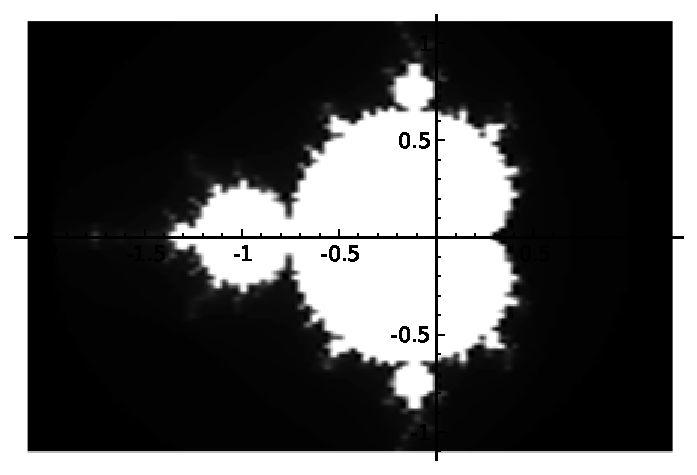
\includegraphics[width=0.8\textwidth]{figures/mandel.pdf} 
\end{center}

\end{frame}


\begin{frame}[fragile]{Letztes Beispiel I}
\begin{sagein}
def Gadisch(x,basis):
    """Berechnung der Darstellung einer natuerlichen Zahl 
x zur Basis b. Rueckgabe des Ergebnis als Liste!"""
    #Abfangen der Eingabe
    if not x in ZZ or x < 0 or basis==1: 
        return 'Eingabe nicht korrekt!'
    T = []  # leere Liste 
    while x>0:
        T.append(x%basis) # Rest der Division
        print '%i : %i = %i Rest %i' % (x,basis,floor(x/basis),x%basis)
        x = floor(x/basis) # Teiler setzen
    # Rueckgabe der Liste
    return T
\end{sagein}
\end{frame}

\begin{frame}[fragile]{Letztes Beispiel II}
\begin{sagein}
Gadisch(6,2)
\end{sagein}
\begin{sage}
6 : 2 = 3 Rest 0
3 : 2 = 1 Rest 1
1 : 2 = 0 Rest 1
[0, 1, 1]
\end{sage}

\begin{sagein}
Gadisch(3.4,2)
\end{sagein}
\begin{sage}
'Eingabe nicht korrekt!'
\end{sage}


\end{frame}

\begin{frame}{Allerletztes Beispiel: Kochsche Kurven I}
\begin{itemize}
\item Seien $y_1,y_2$ zwei Punkte im $\mathbb{R}^2$. 
\item Betrachte die Strecke mit Endpunkten $y_1$ und $y_2$.  
\item Ersetze  diese Strecke durch 4 Strecken 
$\overline{y_1 z_1}$, $\overline{z_1 z_2}$, $\overline{z_2 z_3}$,
$\overline{z_3 y_2}$ mit Endpunkten 
\begin{eqnarray*}
 z_1 &=&\frac23 y_1 + \frac13 y_2\\[0.5cm]
 z_2 &=& \frac{\sqrt{3}}{6} \left( \begin{array}{cc}
 0 & 1 \\ -1 & 0 \\
 \end{array} \right)
 (y_1 - y_2) + \frac12 (y_1 + y_2)\\[0.5cm]
 z_3 &=&\frac13 y_1 + \frac23 y_2
\end{eqnarray*}
\item Dieses Prozedere wird nun für jede einzelne Teilstrecke wiederholt.
\end{itemize}
\end{frame}

\begin{frame}[fragile]{Allerletztes Beispiel II}
\begin{sagein}
def koch(y1,y2,lev):
    Listelinien = []
    if (lev == 0):
        Listelinien.append(line([(y1[0],y1[1]),(y2[0],y2[1])]))
    else:
        # Definieren der neuen Punkte 
        z1 = 2/3 * y1 + 1/3 * y2
        z3 = 1/3 * y1 + 2/3 * y2
        z2 = sqrt(3)/6*matrix([[0, 1],[ -1, 0]])*(y1-y2) + 1/2 * (y1 + y2)
        # Definieren der 4 Strecken
        Listelinien.append(koch(y1, z1, lev-1))
        Listelinien.append(koch(z1, z2, lev-1))
        Listelinien.append(koch(z2, z3, lev-1))
        Listelinien.append(koch(z3, y2, lev-1))
    return add(Listelinien)
\end{sagein}
\end{frame}

\begin{frame}[fragile]{Allerletztes Beispiel III}
\begin{sagein}
# Einfacher Fall einer Linie 
koch(vector([0,0]),vector([1,0]),4)
\end{sagein}
\begin{center}
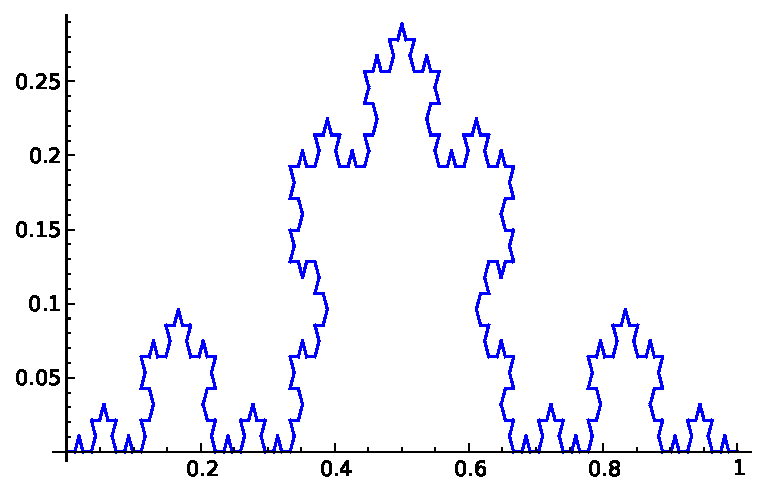
\includegraphics[width=0.7\textwidth]{figures/koch.pdf} 
\end{center}
\end{frame}
\end{document}
